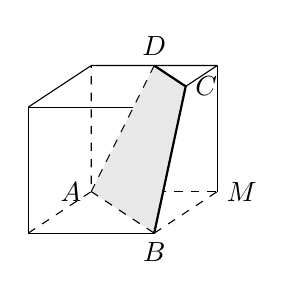
\begin{tikzpicture}[>=stealth, scale=1.6, line join=round]
  % 投影：x 向右、y 向右上（景深）、z 向上
  \def\px#1#2#3{#1+0.5*#2}
  \def\py#1#2#3{#3+0.33*#2}
  % 立方体八个顶点
  \coordinate (FBL) at (0,0);
  \coordinate (BBL) at (0.5,0.33);   % A
  \coordinate (FBR) at (1,0);        % B
  \coordinate (BBR) at (1.5,0.33);   % M
  \coordinate (FTL) at (0,1);
  \coordinate (BTL) at (0.5,1.33);
  \coordinate (FTR) at (1,1);
  \coordinate (BTR) at (1.5,1.33);
  % 可见棱（实线）
  \draw (FBL)--(FBR)--(FTR)--(FTL)--cycle;
  \draw (FTL)--(BTL)--(BTR)--(FTR);
  \draw (BTR)--(BBR);
  % 不可见棱（虚线）
  \draw[dashed] (FBL)--(BBL)--(BTL);
  \draw[dashed] (BBL)--(BBR);
  \draw[dashed] (FBR)--(BBR);
  % 截面：C、D 为两条棱中点，A、B、M 为顶点
  \coordinate (C) at (1.25,1.165);
  \coordinate (D) at (1.0,1.33);
  \fill[gray!18] (0.5,0.33)--(1,0)--(1.25,1.165)--(1.0,1.33)--cycle;
  \draw[dashed] (0.5,0.33)--(1,0);
  \draw[dashed] (0.5,0.33)--(1.0,1.33);
  \draw[thick] (1,0)--(1.25,1.165)--(1.0,1.33);
  % 标注
  \node[left] at (0.5,0.33) {$A$};
  \node[below] at (1,0) {$B$};
  \node[right] at (1.5,0.33) {$M$};
  \node[right] at (1.25,1.165) {$C$};
  \node[above] at (1.0,1.33) {$D$};
\end{tikzpicture}
